% Created 2017-12-10 Sun 22:04
\documentclass[11pt]{article}
\usepackage[utf8]{inputenc}
\usepackage[T1]{fontenc}
\usepackage{fixltx2e}
\usepackage{graphicx}
\usepackage{longtable}
\usepackage{float}
\usepackage{wrapfig}
\usepackage{rotating}
\usepackage[normalem]{ulem}
\usepackage{amsmath}
\usepackage{textcomp}
\usepackage{marvosym}
\usepackage{wasysym}
\usepackage{amssymb}
\usepackage{hyperref}
\tolerance=1000
\usepackage{minted}
\usepackage{fancyhdr}
\setcounter{secnumdepth}{-1} 
\pagestyle{fancy}
\fancyhead{} 
\rhead{\textit{Michael Laufer}}
\lhead{\textit{Numerical Methods Fall 2017, HW6}}
\small

\author{Michael Laufer}
\date{\today}
\title{HW5 Numerical Methods Fall 2017}
\hypersetup{
  pdfkeywords={},
  pdfsubject={},
  pdfcreator={Emacs 25.3.1 (Org mode 8.2.10)}}
\begin{document}

\maketitle
\section{Euler Explicit}
\label{sec-1}
\subsection{Problem}
\label{sec-1-1}
Given the 1D heat conduction equation with no source term:
\[
\frac{ \partial \phi }{ \partial t} = \frac{ \partial^{2} \phi }{ \partial x^{2} }  
\]
given the initial condition:
\[
\phi (t,0) = 1
\]
and the boundary conditions:
\[
\frac{ \partial \phi }{ \partial x } ( t,0) = 0
\]

\[
\frac{ \partial \phi }{\partial x} ( t,1) = - \phi (t,1)
\]

The analytical solution to the problem is given by:
\[
\phi (t,x) = \sum_{n=1}^{\infty} C_{n} exp(- \lambda_{n}^{2} t) \cos ( \lambda_{n} x) 
\]
where:
\[
C_{n}= \frac{4 \sin \lambda_{n}}{2 \lambda_{n} + 2 \sin (2 \lambda_{n})}
\]

We will use the explicit (forward Euler) method to solve the problem numerically. For our purposes, it is sufficient to use just the first four terms of $C_{n}$ for an accurate enough answer.

\subsection{Forward Euler Scheme}
\label{sec-1-2}
The governing equation is discretized using a second order central-differencing for the spatial derivative for the interior nodes, and a first order forward differencing scheme for the temporal derivative.
The second order central-differencing for the spatial derivative:
\[
\frac{ \partial^{2} \phi }{ \partial x^{2} } = \frac{\phi_{i+1} -2 \phi_{i} + \phi_{i-1}}{( \Delta x)^{2} }
\]
First order forward difference for temporal derivative:
\[
\frac{ \partial \phi }{ \partial t} = \frac{\phi_{i,n+1} - \phi_{i,n}}{\Delta t}
\]
Rearranging for $\phi_{i,n+1}$ leads to the scheme:
\[
\phi_{i,n+1} = \phi_{i,n} + \Delta t \left[ \frac{\phi_{i+1,n} -2 \phi_{i,n} + \phi_{i-1,n}}{( \Delta x)^{2} } \right]
\]
Regarding the boundary conditions, we will perform a first order forward/backward differencing to the boundary equations:
\[
\frac{ \partial \phi }{ \partial x } ( t,0) = 0
\]
hence:
\[
\frac{\phi_{2,n+1} - \phi_{1,n}}{\Delta x} = 0 \implies \phi_{1,n+1}=\phi_{2,n}
\]

\[
\frac{ \partial \phi }{\partial x} ( t,1) = - \phi (t,1)
\]
hence 
\[
\frac{\phi_{m,n+1}-\phi_{m-1,n}}{\Delta x} = - \phi_{m,n} \implies \phi_{m,n+1} = -\Delta x \phi_{m-1,n} + \phi_{m,n} 
\]
The stability criterion for the forward Euler method is given by:
\[
\Delta t \leq \frac{1}{2} \frac{(\Delta x)^{2}}{\alpha}
\]
Choosing 26 nodes in the x-direction leads to a maximum stable time step of: $\Delta t_{max} \leq 0.0008$
We will choose to use a time step of $\frac{1}{2} \Delta t_{max} = 0.0004$ sec. 

\subsection{Results}
\label{sec-1-3}
The equations are solved with a time-marching approach, and results were recorded at times $t = 0.1, 0.2, 0.4, 0.8$ and plotted on a single graph.

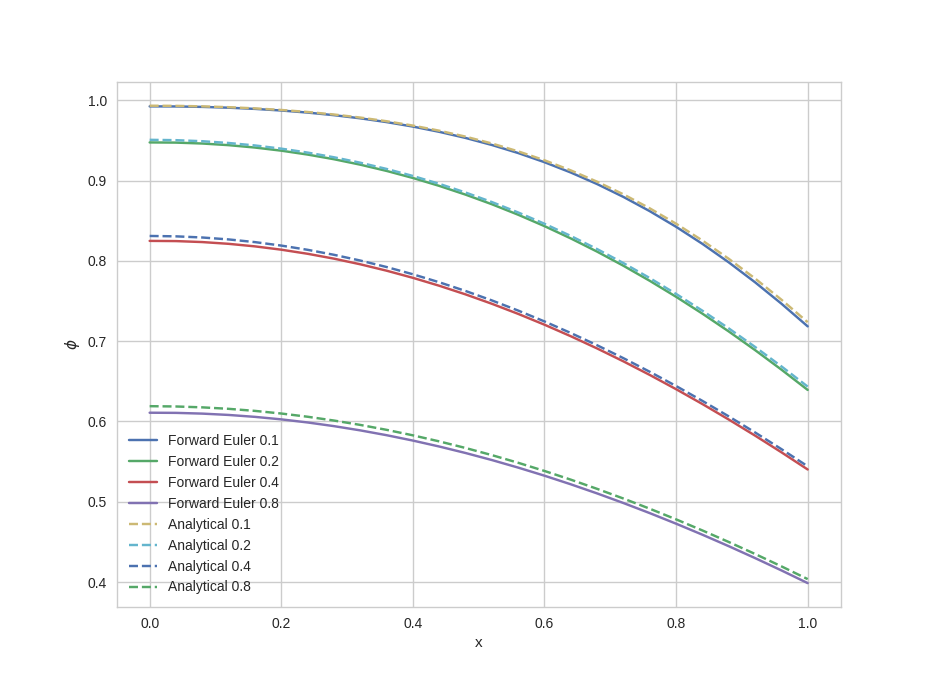
\includegraphics[width=14cm]{./figures/phi.png}

\subsection{Discussion}
\label{sec-1-4}
It is clear that a good agreement is seen between the analytical solution and the numerical one. But we can observe that the numerical solution drifts from the analytical as more time passes.  
Choosing a higher order time-stepping method such as the Crank-Nicholson method should help reduce this error. Alternatively, the time-step can be further reduced.

\newpage
\section{Appendix: Python Code}
\label{sec-2}
\begin{minted}[]{python}
import numpy as np
import matplotlib.pyplot as plt
import seaborn as sns
sns.set_style('whitegrid')

if __name__ == "__main__":
    # parameters
    nx = 26
    dx = 1.0 / (nx - 1)
    dt = 0.25*(dx**2)
    finaltime = 1.0

    x = np.linspace(0,1,nx)
    nt = int(finaltime/dt)
    dx2 = dx**2
    phi = np.ones(nx, dtype=float)

    for n in range(1,nt):
	phi_n = phi.copy()
	phi[1:-1] = phi_n[1:-1] + (dt/dx2)*(phi_n[2:] -2*phi_n[1:-1] + phi_n[0:-2])
	phi[0] = phi_n[1]
	phi[-1] = -dx*phi_n[-1] + phi_n[-2]

	if n*dt == 0.1:
	    phi_01 = phi.copy()
	elif n*dt == 0.2:
	    phi_02 = phi.copy()
	elif n*dt == 0.4:
	    phi_04 = phi.copy()
	elif n*dt == 0.8:
	    phi_08 = phi.copy()

    lamb = np.array([0.8603, 3.4256, 6.4373, 9.5293])
    Cn = (4*np.sin(lamb))/(2*lamb + np.sin(2*lamb))
    phi_anal = np.zeros((nt,nx))
    for n in range(nt):
	phi_anal[n] = Cn[0]*np.exp((-(lamb[0]**2))*n*dt)*np.cos(lamb[0]*x) +\
		      Cn[1]*np.exp((-(lamb[1]**2))*n*dt)*np.cos(lamb[1]*x) +\
		      Cn[2]*np.exp((-(lamb[2]**2))*n*dt)*np.cos(lamb[2]*x) +\
		      Cn[3]*np.exp((-(lamb[3]**2))*n*dt)*np.cos(lamb[3]*x)

    plt.plot(x, phi_01, label='Forward Euler 0.1')
    plt.plot(x, phi_02, label='Forward Euler 0.2')
    plt.plot(x, phi_04, label='Forward Euler 0.4')
    plt.plot(x, phi_08, label='Forward Euler 0.8')
    plt.plot(x, phi_anal[int(0.1/dt)], '--', label='Analytical 0.1')
    plt.plot(x, phi_anal[int(0.2/dt)], '--', label='Analytical 0.2')
    plt.plot(x, phi_anal[int(0.4/dt)], '--', label='Analytical 0.4')
    plt.plot(x, phi_anal[int(0.8/dt)], '--', label='Analytical 0.8')
    plt.xlabel('x')
    plt.ylabel(r'$\phi$')    
    plt.legend()
    plt.show()
\end{minted}
% Emacs 25.3.1 (Org mode 8.2.10)
\end{document}